% Created 2026-03-20 Fri 12:51
% Intended LaTeX compiler: lualatex
\documentclass[xcolor=table,10pt,aspectratio=169]{beamer}

\RequirePackage[l2tabu,orthodox]{nag}            %% Warn about obsolete commands and packages
\RequirePackage{amsmath,amsfonts,amssymb,amsthm} %% Math
\RequirePackage{ifpdf,ifxetex,ifluatex}          %% Detect XeTeX and LuaTeX
\RequirePackage{xspace}
\RequirePackage{graphicx}
\RequirePackage{comment}
\RequirePackage{url}
\RequirePackage{relsize}
\RequirePackage{booktabs}
\RequirePackage{tabularx}
\RequirePackage[normalem]{ulem}
\ifluatex%
\else%
  \RequirePackage[all]{xy}
\fi%
\RequirePackage{etoolbox}
\RequirePackage{csquotes}
\RequirePackage[export]{adjustbox}

\RequirePackage{silence}
\WarningsOff[microtype]
\WarningFilter{microtype}{Unknown slot}

% https://tex.stackexchange.com/questions/64459/overfull-vbox-warning-disable
\vfuzz=30pt
\hfuzz=30pt


%%%
%%% Code Listings
%%%

\RequirePackage{listings}
\lstdefinelanguage{Sage}[]{Python}{morekeywords={True,False,sage,cdef,cpdef,ctypedef,self},sensitive=true}
\lstdefinelanguage{jupyter-python}[]{Python}{morekeywords={True,False,self},sensitive=true}

\lstset{frame=none,
  showtabs=False,
  showspaces=False,
  showstringspaces=False,
  commentstyle={\color{gray}},
  keywordstyle={\color{mLightBrown}\textbf},
  stringstyle ={\color{mDarkBrown}},
  frame=single,
  basicstyle=\tt\scriptsize\relax,
  backgroundcolor=\color{gray!190!black},
  inputencoding=utf8,
  literate={…}{{\ldots}}1,
  belowskip=0.0em,
}

\makeatletter
\patchcmd{\@verbatim}
  {\verbatim@font}
  {\verbatim@font\scriptsize}
  {}{}
\makeatother


%%%
%%% Pseudocode
%%%

\let\nl\undefine
\let\procedure\relax
\let\endprocedure\relax
\usepackage{algorithm2e}

%%%
%%% Tikz
%%%

\RequirePackage{tikz,pgfplots}
\pgfplotsset{compat=newest}

\usetikzlibrary{calc}
\usetikzlibrary{arrows}
\usetikzlibrary{automata}
\usetikzlibrary{positioning}
\usetikzlibrary{decorations.pathmorphing}
\usetikzlibrary{backgrounds}
\usetikzlibrary{fit,}
\usetikzlibrary{shapes.symbols}
\usetikzlibrary{chains}
\usetikzlibrary{shapes.geometric}
\usetikzlibrary{shapes.arrows}
\usetikzlibrary{graphs}

%% Cache but disable by default

\usetikzlibrary{external}
\tikzset{external/export=false}

\definecolor{DarkPurple}{HTML}{332288}
\definecolor{DarkBlue}{HTML}{6699CC}
\definecolor{LightBlue}{HTML}{88CCEE}
\definecolor{DarkGreen}{HTML}{117733}
\definecolor{DarkRed}{HTML}{661100}
\definecolor{LightRed}{HTML}{CC6677}
\definecolor{LightPink}{HTML}{AA4466}
\definecolor{DarkPink}{HTML}{882255}
\definecolor{LightPurple}{HTML}{AA4499}
\definecolor{DarkBrown}{HTML}{604c38}
\definecolor{DarkTeal}{HTML}{23373b}
\definecolor{LightBrown}{HTML}{EB811B}
\definecolor{LightGreen}{HTML}{14B03D}
\definecolor{DarkOrange}{HTML}{FFDD00}

\pgfplotsset{width=1.0\textwidth,
  height=0.6\textwidth,
  cycle list={%
    solid,LightGreen,thick\\%
    dotted,LightRed,very thick\\%
    dashed,DarkBlue,thick\\%
    dashdotted,DarkPink,thick\\%
    dashdotdotted,LightGreen,thick\\%
    loosely dotted,very thick\\%
    loosely dashed,DarkBlue,very thick\\%
    loosely dashdotted,DarkPink,very thick\\%
    \\%
    DarkBrown,thick\\%
  },
  legend pos=north west,
  legend cell align={left}}

\pgfplotsset{select coords between index/.style 2 args={
    x filter/.code={
        \ifnum\coordindex<#1\def\pgfmathresult{}\fi
        \ifnum\coordindex>#2\def\pgfmathresult{}\fi
    }
}}

\setlength{\marginparwidth}{2cm}
\pgfplotsset{compat=1.18}

%%%
%%% SVG (Inkscape)
%%%

\ifpdf% 
\providecommand{\executeiffilenewer}[3]{%
  \ifnum\pdfstrcmp{\pdffilemoddate{#1}}%
    {\pdffilemoddate{#2}}>0%
    {\immediate\write18{#3}}
  \fi%
}
\else%
\providecommand{\executeiffilenewer}[3]{%
  {\immediate\write18{#3}} % hack
}
\fi%

\providecommand{\includesvg}[2][1.0\textwidth]{%
 \executeiffilenewer{#1.svg}{#1.pdf}%
 {inkscape -z -D --file=#2.svg --export-pdf=#2.pdf --export-latex --export-area-page}%
 \def\svgwidth{#1} 
 \input{#2.pdf_tex}%
} 

%%%
%%% Attachments
%%%

\RequirePackage{embedfile}


%%%
%%% Metropolis Theme
%%%

\usetheme{metropolis}
\metroset{color/block=fill}
\metroset{numbering=none}
\metroset{outer/progressbar=foot}
\metroset{titleformat=smallcaps}

\setbeamercolor{description item}{fg=mLightBrown}
\setbeamerfont{footnote}{size=\scriptsize}
\setbeamercolor{example text}{fg=mDarkBrown}
\setbeamercolor{block title alerted}{fg=white, bg=mDarkBrown}
\setbeamerfont{alerted text}{series=\ifmmode\boldmath\else\bfseries\fi}

\definecolor{gamechangecolor}{HTML}{f8e8c6}

\renewcommand*{\UrlFont}{\ttfamily\relax}

%%%
%%% UTF-8 & Fonts
%%% 

% \RequirePackage{unicodesymbols} % after metropolis which loads fontspec

\ifboolexpr{bool{xetex} or bool{luatex}}{%
\setmonofont[BoldFont={Cousine Bold},
             ItalicFont={Cousine Italic},
             BoldItalicFont={Cousine Bold Italic},
             Scale=0.9]{Cousine}             
}{%
}

%%%
%%% BibLaTeX
%%%

\RequirePackage[backend=bibtex,
            style=alphabetic,
            maxnames=8,maxbibnames=8,maxalphanames=8,
            citestyle=alphabetic]{biblatex}

\bibliography{local.bib,abbrev3.bib,crypto_crossref.bib,rfc.bib,jacm.bib,dcc.bib}

\setbeamertemplate{bibliography item}[text]
% https://tex.stackexchange.com/questions/683533/beamer-theme-metropolis-does-not-allow-different-font-size-for-fullcite
\setbeamerfont{bibliography entry title}{size=}
\setbeamerfont{bibliography entry author}{size=}
\setbeamerfont{bibliography entry location}{size=}
\setbeamerfont{bibliography entry note}{size=}

\DeclareFieldFormat{title}{\alert{#1}}
\DeclareFieldFormat[book]{title}{\alert{#1}}
\DeclareFieldFormat[thesis]{title}{\alert{#1}}
\DeclareFieldFormat[inproceedings]{title}{\alert{#1}}
\DeclareFieldFormat[incollection]{title}{\alert{#1}}
\DeclareFieldFormat[article]{title}{\alert{#1}}
\DeclareFieldFormat[misc]{title}{\alert{#1}}

%%% 
%%% Microtype
%%%

\IfFileExists{upquote.sty}{\RequirePackage{upquote}}{}
%% https://github.com/schlcht/microtype/issues/43
%% \IfFileExists{microtype.sty}{\RequirePackage{microtype}}{}
%% \IfFileExists{microtype.sty}{\PassOptionsToPackage{verbose=silent}{microtype}}{}

\setlength{\parindent}{0pt}                   %%
\setlength{\parskip}{6pt plus 2pt minus 1pt}  %%
\setlength{\emergencystretch}{3em}            %% prevent overfull lines
\setcounter{secnumdepth}{0}                   %%

%%%
%%% Maths
%%%

\DeclareMathOperator{\Vol}{Vol}
\DeclareMathOperator{\vol}{vol}
\DeclareMathOperator{\GH}{GH}
\renewcommand{\vec}[1]{\ensuremath{\mathbf{#1}}\xspace}
\newcommand{\norm}[1]{\left\lVert#1\right\rVert}
\providecommand{\mat}[1]{\ensuremath{\vec{#1}}\xspace}
\providecommand{\ring}[0]{\ensuremath{\mathcal{R}}\xspace}

\usepackage{amsmath}
\usepackage{fontspec}
\usepackage{graphicx}
\usepackage{longtable}
\usepackage{wrapfig}
\usepackage{rotating}
\usepackage[normalem]{ulem}
\usepackage{capt-of}
\usepackage{hyperref}
\usepackage{booktabs}
\usepackage{newunicodechar}
\usepackage[notions,operators,sets,keys,ff,adversary,primitives,complexity,asymptotics,lambda,landau,advantage]{cryptocode}
\usepackage[capitalize]{cleveref}
\usepackage[,]{stmaryrd}
\usepackage[british]{babel}
\usepackage{xspace}
\usepackage{units}
\usepackage{nicefrac}
\usepackage{gensymb}
\usepackage{amsthm}
\usepackage{amsmath}
\usepackage{amssymb}
\usepackage{xcolor}
\usepackage{listings}
\usepackage[color=cyan!0!magenta!4!yellow!16]{todonotes}
\PassOptionsToPackage{british}{babel}
\newtheorem{assumption}{Assumption}
\mathchardef\mhyphen="2D
\newcommand{\SIS}{\ensuremath{\mathsf{SIS}}\xspace}
\newcommand{\ISIS}{\ensuremath{\mathsf{ISIS}}\xspace}
\newcommand{\HISIS}{\ensuremath{\mathsf{H\pcmathhyphen{}ISIS}}\xspace}
\newcommand{\HSIS}{\ensuremath{\mathsf{H\pcmathhyphen{}SIS}}\xspace}
\newcommand{\params}{\mathsf{params}}
\newcommand{\DIST}{\pcalgostyle{Dist}}
\newcommand{\Exp}{\mathsf{Exp}}
\newcommand{\ball}[2]{\ensuremath{\mathsf{B}^{#1}{(#2)}}}
\usetheme{default}
\author{Martin R. Albrecht}
\date{ICQCS'26 (20 March 2026)}
\title{The space-time hardness of lattice problems}
\hypersetup{
pdfauthor={Martin R. Albrecht},
pdftitle={The space-time hardness of lattice problems},
pdfkeywords={},
pdfsubject={},
pdfcreator={},
pdflang={English},
colorlinks,
citecolor=gray,
filecolor=gray,
linkcolor=gray,
urlcolor=gray
}
\usepackage[backend=bibtex]{biblatex}

\begin{document}

\maketitle
\begin{frame}[label={sec:orgedbd1b3}]{Hardness of hinted ISIS from the space-time hardness of lattice problems}
\begin{columns}
\begin{column}{0.5\columnwidth}
\begin{center}
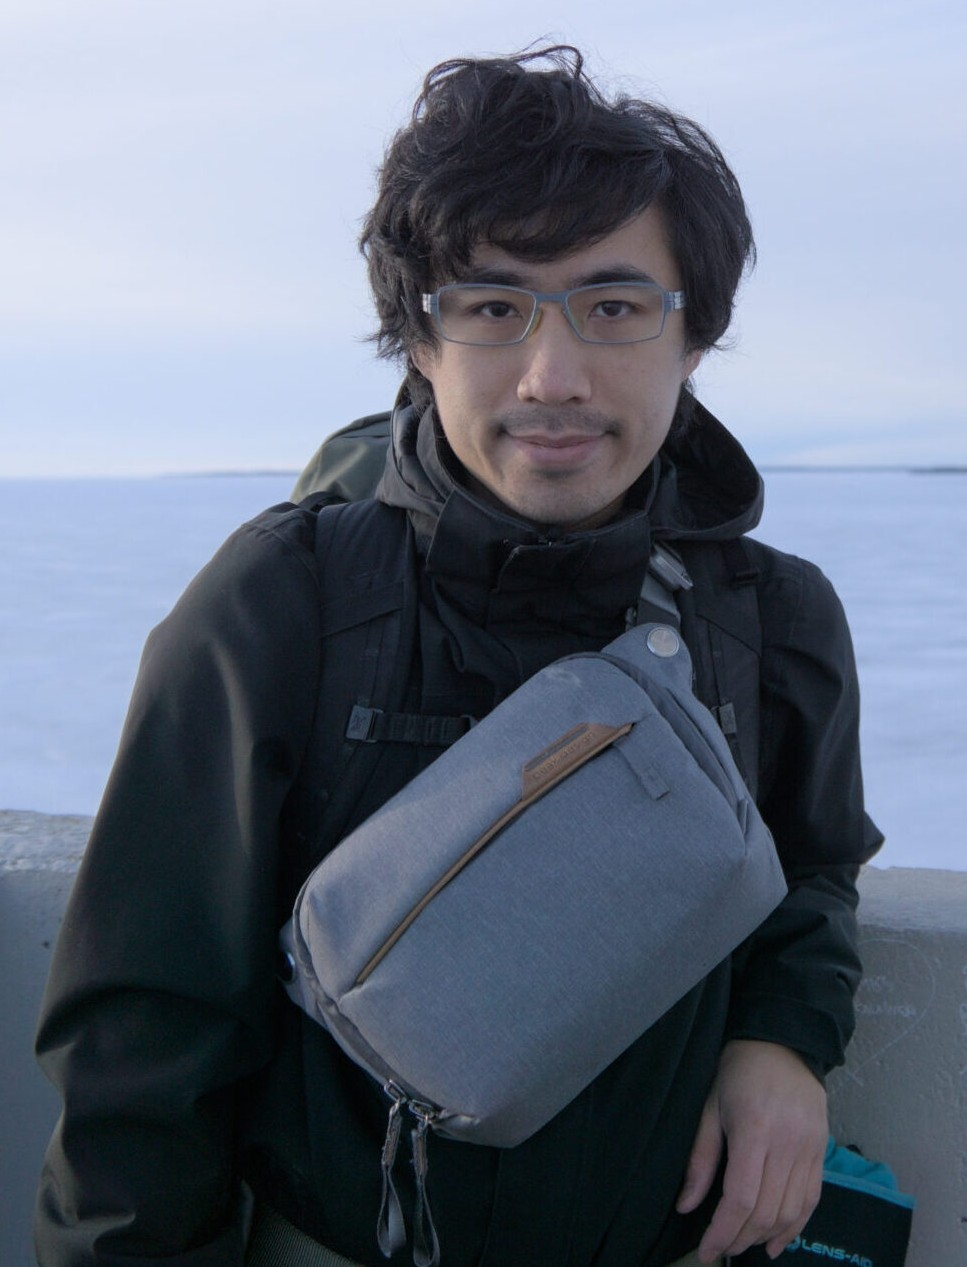
\includegraphics[keepaspectratio,frame,height=0.6\textheight]{./assets/russell.jpg}
\end{center}
\end{column}
\begin{column}{0.5\columnwidth}
\begin{center}
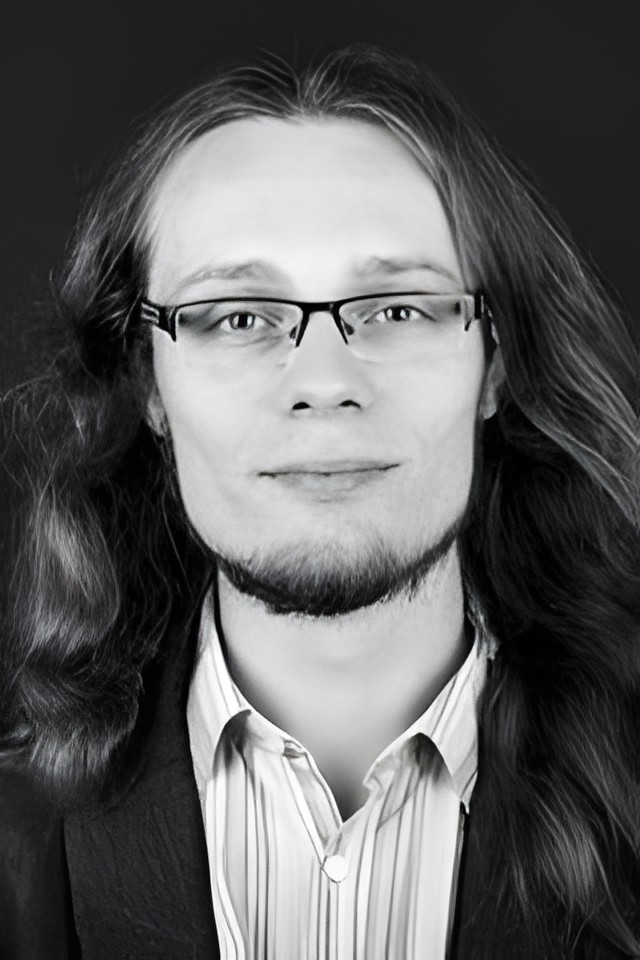
\includegraphics[keepaspectratio,frame,height=0.6\textheight]{./assets/eamonn.jpg}
\end{center}
\end{column}
\end{columns}
\begin{center}
joint work with Russell W. F. Lai and Eamonn W. Postlethwaite\\
\url{https://ia.cr/2026/187}
\end{center}
\end{frame}
\begin{frame}[label={sec:org07f6be9}]{Motivation for those who like applications: Don't sign it twice!}
\begin{columns}
\begin{column}{0.65\columnwidth}
\begin{center}
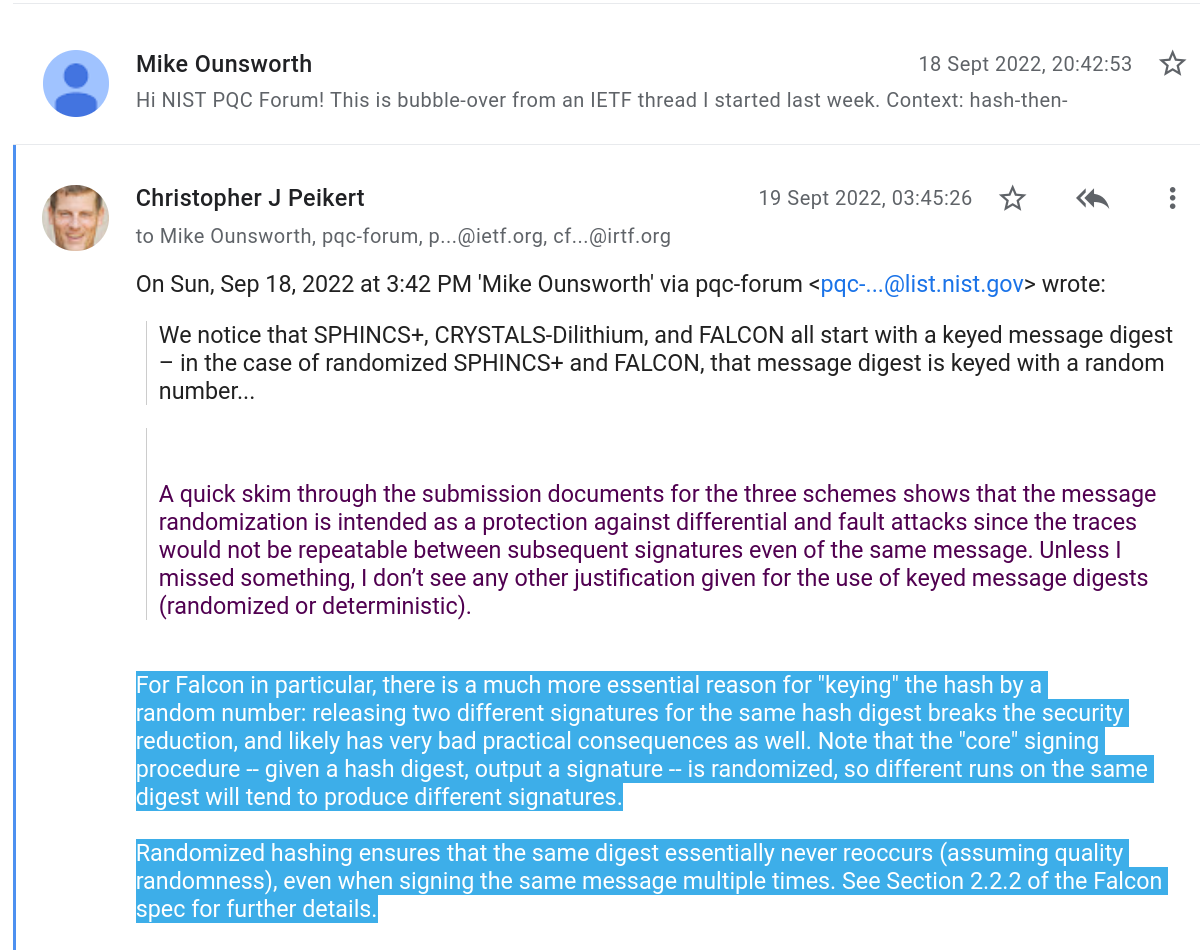
\includegraphics[keepaspectratio,frame,height=.8\textheight]{./assets/falcon-stark-warning.png}
\end{center}

{\tiny \url{https://groups.google.com/a/list.nist.gov/g/pqc-forum/c/cIsc6tUY9Rw/m/E0fPG7QkAQAJ} \par}
\end{column}
\begin{column}{0.35\columnwidth}
\alert{verification key}

\(\mat{A} \in \ZZ_{q}^{n \times m}\)

\alert{signing key}

short \(\mat{T}\) s.t. \(\mat{A} \cdot \mat{T} \equiv \mat{0} \bmod q\)

\alert{signature}

\((\vec{u},r)\) s.t. \(H(m,r) \equiv \mat{A} \cdot \vec{u} \bmod q\) with \(\vec{u}\) short
\end{column}
\end{columns}
\end{frame}
\begin{frame}[label={sec:org16224f5}]{Motivation for those who like lattices: An enticing lie}
\begin{center}

\includegraphics[keepaspectratio,frame,height=.8\textheight]{./assets/sis-with-hints-teaser.jpg}
\end{center}
\end{frame}
\section{Efficient Adversaries}
\label{sec:orga0bcb66}

\begin{frame}[label={sec:orgf71b901}]{Some lattice problems and their relations}
\begin{definition}[\(\gamma\)-SIVP]
Given \(\gamma \ge 1\) and a full-rank lattice \(\Lambda \subset \RR^{n}\), find linearly independent \(\vec{v}_{1}, \ldots \vec{v}_{n}\) such that \(\max\norm{\vec{v}_i} \leq \gamma \cdot \lambda_{n}(\Lambda)\),  where \(\lambda _{n}(\Lambda)\) is the \(n\)-th successive minimum of ⁠\(\Lambda\).
\label{def:sivp}
\end{definition}

\begin{definition}[SIS (\cite{STOC:Ajtai96})]
Given a random \(\mat{A} \gets \ZZ_{q}^{n \times m}\), return \(\vec{u} \in \ZZ^{m}\) with \(0 < \norm{\vec{u}} \leq \beta\) such that \(\mat{A} \cdot \vec{u} \equiv \vec{0} \bmod q\).
\label{def:sis}
\end{definition}

\begin{theorem}[SIVP \(\implies\) SIS~\cite{STOC:Ajtai96,SIAM:MicReg07}]
Let \(m, \beta \in \poly[n]\), \(q \geq 8\,n\cdot\sqrt{m}\cdot\beta\) and \(\gamma = 8\, \beta\cdot\sqrt{n} \cdot \omega(\sqrt{\log n})\). Then solving SIS for \(n,m,q,\beta\) in time \(\tau\) and memory \(\mu\), solves \(\gamma\)-SIVP in time \(\tau + \poly[n]\) and memory \(\mu + \poly[n]\).
\label{thm:sivp-sis}
\end{theorem}
\end{frame}
\begin{frame}[label={sec:org5a7743a}]{Notation}
Write
\begin{itemize}
\item \(\SIS_{n,m,q,\beta}\) to represent the SIS problem.
\item \((\tau, \mu)\mhyphen\SIS_{n,m,q,\beta}\) for the set of algorithms that solve \(\SIS_{n,m,q,\beta}\) in time \(\tau\), memory \(\mu\) and with non-negligible success probability.
\item \(\Lambda_{q}^{\bot}(\mat{A}) \coloneqq \{\vec{x} \in \ZZ^m : \mat{A} \cdot \vec{x} \equiv \vec{0} \bmod q\}\) for the kernel lattice of \(\mat{A}\). SIS asks to find short elements in this lattice.
\item \(D_{\Lambda,s,\vec{c}}\) for the discrete Gaussian distribution with support \(\Lambda\), parameter \(s\) and centre \(\vec{c}\).
\end{itemize}
\end{frame}
\begin{frame}[label={sec:org0f63eb9}]{"Let \(\adv\) be a \sout{ PPT }BQP adversary …"}
\begin{assumption}[SIS]
For sensible \(m,q,\beta \in \poly[n]\) we have \(\left(\poly[n],\allowbreak \poly[n]\right)\mhyphen\SIS_{n,m,q,\beta} = \emptyset\).
\label{ass:sis}
\end{assumption}
\end{frame}
\begin{frame}[label={sec:orgce28a80}]{"Let \(\adv\) be a subexponential adversary …"}
\begin{assumption}[Subexponential-secure SIS]
For sensible \(m,q,\beta \in \poly[n]\) we have \(\left(2^{o(n)}, 2^{o(n)}\right)\mhyphen\SIS_{n,m,q,\beta} = \emptyset\).
\label{ass:sis-subexponential}
\end{assumption}
\end{frame}
\begin{frame}[label={sec:org311e9dd}]{Algorithms for finding short vectors / solving SIS}
\begin{columns}[t]
\begin{column}{0.5\columnwidth}
\textbf{Enumeration}

\begin{itemize}
\item Search through vectors smaller than a given bound: project down to 1-dim problem, lift to 2-dim problem …
\item \textbf{Time:} \(n^{\Theta(n)}\)
\item \textbf{Memory:} \(\poly[n]\)
\end{itemize}
\end{column}
\begin{column}{0.5\columnwidth}
\textbf{Sieving}

\begin{itemize}
\item Produce new, shorter vectors by considering sums and differences of existing vectors
\item \textbf{Time:} \(2^{\Theta(n)}\)
\item \textbf{Memory:} \(2^{\Theta(n)}\)
\end{itemize}
\end{column}
\end{columns}
\end{frame}
\begin{frame}[label={sec:org07157f4}]{Sieving I}
\tikzset{external/export=true}
\tikzsetnextfilename{sieving-idea-1}
\centering
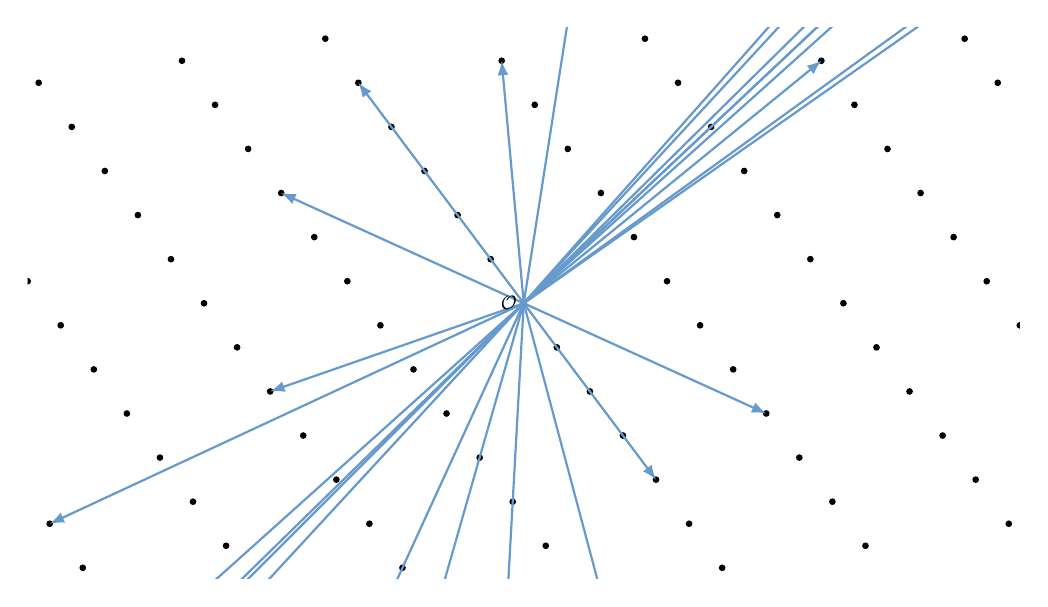
\begin{tikzpicture}[scale=0.7, every node/.style={scale=0.7}]
  \coordinate (Origin)   at (0,0);

  \clip (-9,-5) rectangle (9,5);
  \pgftransformcm{1}{0.6}{0.7}{1}{\pgfpoint{0cm}{0cm}}

  \foreach \x in {-10,-9,...,10}{%
    \foreach \y in {-10,-9,...,10}{%
      \node[draw,circle,inner sep=1pt,fill] at (2*\x,2*\y) {};
    }
  }
  % \draw [ultra thick,-latex,red] (Origin)
  % -- (Bone) node [above left] {$b_1$};
  % \draw [ultra thick,-latex,red] (Origin)
  % -- (Btwo) node [below right] {$b_2$};

  \foreach \x in {-5,-3,2,4,5}{%
    \foreach \y in {-6,-4,1,4,5}{%
      \draw [thick,-latex,DarkBlue] (Origin)
      -- (2*\x,2*\y) {};
    }
  }

  \node [left] at (Origin) {$\mathcal{O}$};
\end{tikzpicture}
\tikzset{external/export=false}
\end{frame}
\begin{frame}[label={sec:orgf57a660}]{Sieving II}
\tikzset{external/export=true}
\tikzsetnextfilename{sieving-idea-2}
\centering
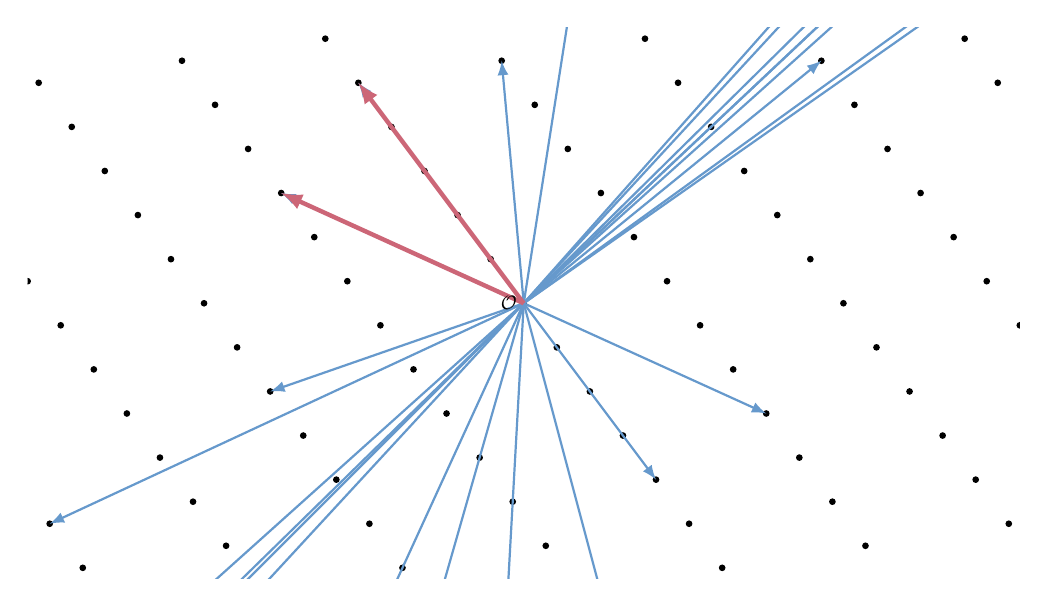
\begin{tikzpicture}[scale=0.7, every node/.style={scale=0.7}]
  \coordinate (Origin)   at (0,0);

  \clip (-9,-5) rectangle (9,5);
  \pgftransformcm{1}{0.6}{0.7}{1}{\pgfpoint{0cm}{0cm}}

  \foreach \x in {-10,-9,...,10}{%
    \foreach \y in {-10,-9,...,10}{%
      \node[draw,circle,inner sep=1pt,fill] at (2*\x,2*\y) {};
    }
  }

  \foreach \x in {-5,-3,2,4,5}{%
    \foreach \y in {-6,-4,1,4,5}{%
      \draw [thick,-latex,DarkBlue] (Origin)
      -- (2*\x,2*\y) {};
    }
  }

  \draw [ultra thick,-latex,LightRed] (Origin) -- (-10,10) {};
  \draw [ultra thick,-latex,LightRed] (Origin) -- (-10,8) {};

  \node [left] at (Origin) {$\mathcal{O}$};
\end{tikzpicture}
\tikzset{external/export=false}
\end{frame}
\begin{frame}[label={sec:orgc2c8950}]{Sieving III}
\tikzset{external/export=true}
\tikzsetnextfilename{sieving-idea-3}
\centering
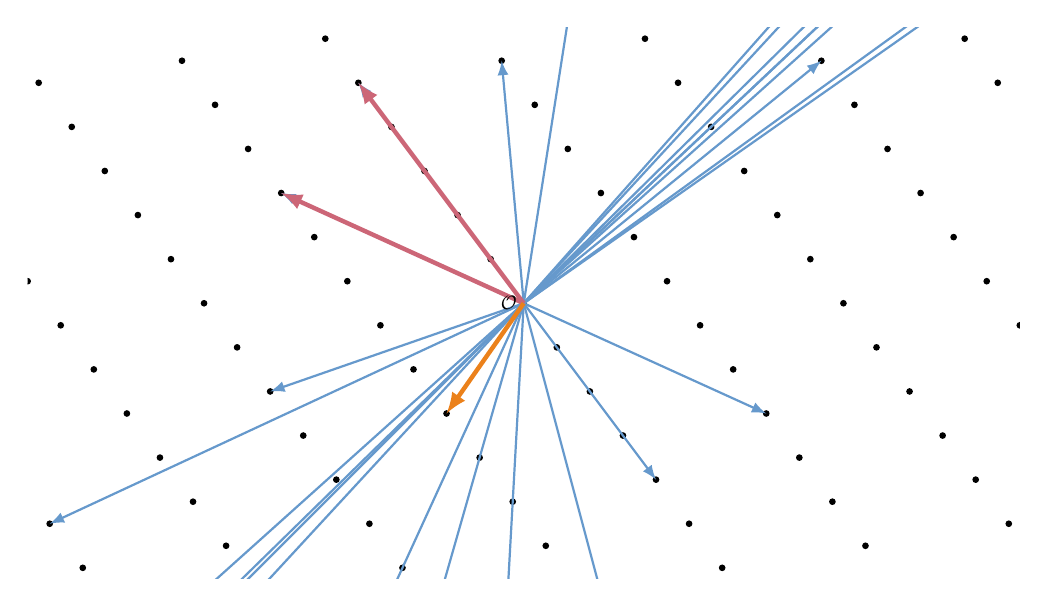
\begin{tikzpicture}[scale=0.7, every node/.style={scale=0.7}]
  \coordinate (Origin)   at (0,0);

  \clip (-9,-5) rectangle (9,5);
  \pgftransformcm{1}{0.6}{0.7}{1}{\pgfpoint{0cm}{0cm}}

  \coordinate (Bone) at (0,2);
  \coordinate (Btwo) at (2,-2);

  \foreach \x in {-10,-9,...,10}{%
    \foreach \y in {-10,-9,...,10}{%
      \node[draw,circle,inner sep=1pt,fill] at (2*\x,2*\y) {};
    }
  }

  \foreach \x in {-5,-3,2,4,5}{%
    \foreach \y in {-6,-4,1,4,5}{%
      \draw [thick,-latex,DarkBlue] (Origin)
      -- (2*\x,2*\y) {};
    }
  }

  \draw [ultra thick,-latex,LightRed] (Origin) -- (-10,10) {};
  \draw [ultra thick,-latex,LightRed] (Origin) -- (-10,8) {};
  \draw [ultra thick,-latex,LightBrown] (Origin) -- (0,-2) {};

  \node [left] at (Origin) {$\mathcal{O}$};
\end{tikzpicture}
\tikzset{external/export=false}
\end{frame}
\begin{frame}[label={sec:orgcd30482}]{Space-time hardness: cryptanalysis}
\begin{itemize}
\item "It is still unclear if we can get a \(2^{O(n)}\) algorithm that uses only polynomial space" \footfullcite{SODA:MicVou10}
\item "is it possible to achieve exponential time complexity with a polynomially bounded space requirement?" \footfullcite{HanPujSte11}
\item "A more general open problem is whether SVP can be solved in singly exponential time but only polynomial space." \footfullcite{STOC:ADRS15}
\end{itemize}
\end{frame}
\begin{frame}[label={sec:orgb64a99c}]{Space-time hardness: conjecture}
\begin{center}
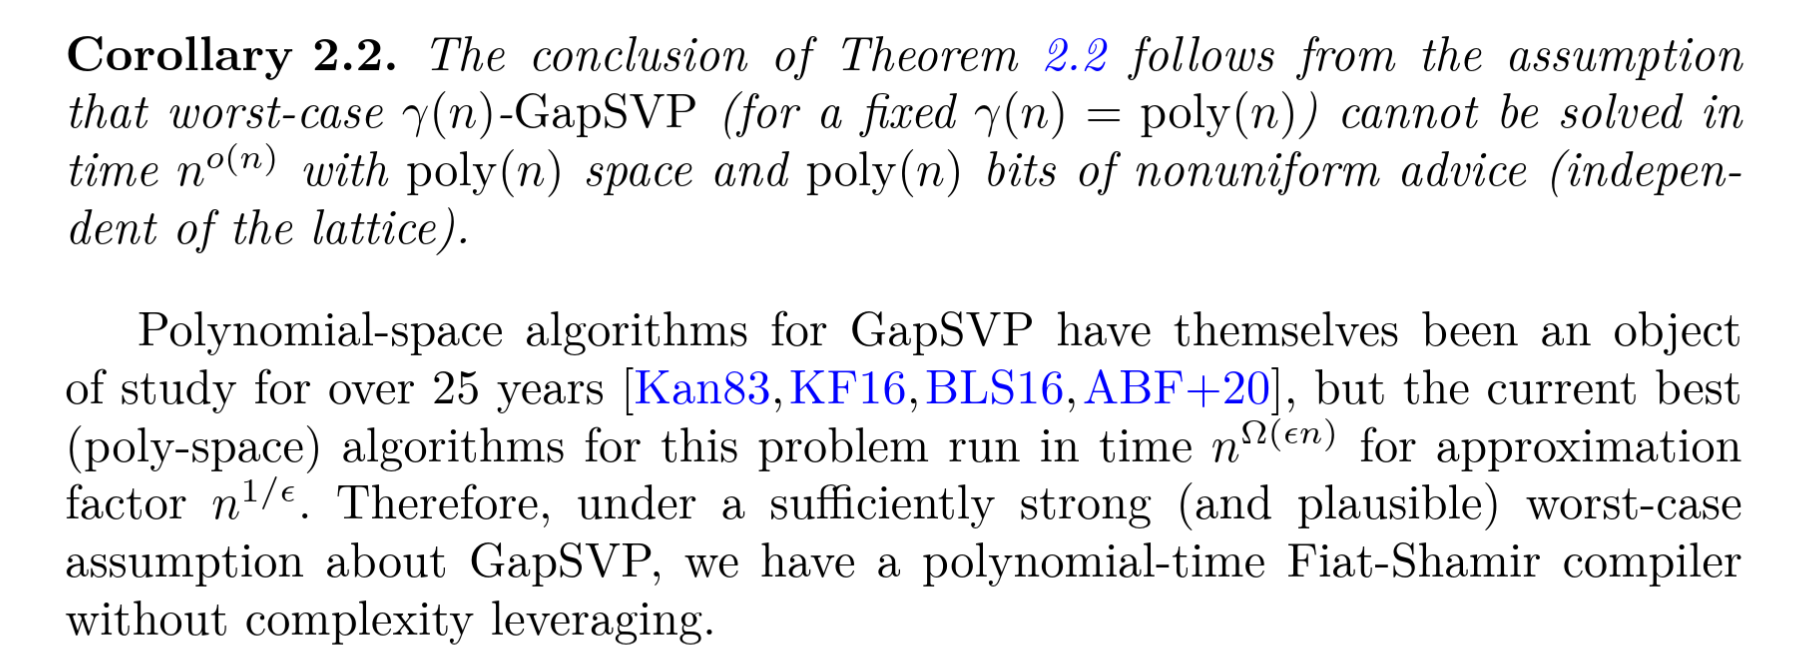
\includegraphics[keepaspectratio,frame,height=.6\textheight]{./assets/conjecture-space-time-hardness.png}
\end{center}

{\footnotesize \fullcite{C:LomVai20} \par}
\end{frame}
\begin{frame}[label={sec:org1e83816}]{A corollary}
\begin{assumption}[Space-time hard SIS]
For sensible \(m,q,\beta \in \poly[n]\) we have \(\left(2^{O(n)}, \poly[n]\right)\mhyphen\SIS_{n,m,q,\beta} = \emptyset\).
\label{ass:space-time-sis}
\end{assumption}
\end{frame}
\begin{frame}[label={sec:org1eefe10}]{A corollary (a specialisation)}
\begin{assumption}[Space-time hard SIS]
For sensible \(q,\beta \in \poly[n]\), \(m \in O(n)\) we have \(\left(\alert{\mathbf{2^{O(m)}}}, \poly[n]\right)\mhyphen\SIS_{n,m,q,\beta} = \emptyset\).
\label{ass:space-time-sis-m}
\end{assumption}

\begin{itemize}
\item When \(m \leq O(n)\) then \(2^{O(n)} = 2^{O(m)}\); we consider only this case in this talk.
\item In the paper we also consider \(m \leq o(n \log n)\), which is covered by the conjecture.
\item When \(m \ge \Omega(n \log n)\), there are algorithms in \(\left(2^{O(m)}, \poly[n]\right)\mhyphen\SIS_{n,m,q,\beta}\).
\end{itemize}
\end{frame}
\section{Hinted lattice problems}
\label{sec:org483ed9b}
\begin{frame}[label={sec:org66937a6}]{H-SIS}
\begin{columns}
\begin{column}{0.4\columnwidth}
\centering
\begin{pchstack}[center]
    \procedure[mode=text]{$\Exp\mhyphen\HISIS_{(k, m, q, \beta, s),\adv}(1^n)$}{
        \((\mat{A}, \vec{t}) \gets \ZZ_q^{n\times m} \times \ZZ_q^n\)\\
        \((\vec{u}_1, \dots, \vec{u}_k) \gets D_{\Lambda_q^\bot(\mat{A}),s,\vec{0}}\) \pccomment{\(\norm{\vec{u}_i} \approx s \sqrt{m}\)}\\
        \(\vec{u} \gets{} \adv(\mat{A}, \vec{t}, \vec{u}_1, \dots, \vec{u}_k)\)\\
        \pcreturn{ \(\llbracket{} \mat{A} \cdot \vec{u} = \vec{t} \land \norm{\vec{u}} \leq \beta \rrbracket{} \)}
    }
\end{pchstack}
\end{column}
\begin{column}{0.6\columnwidth}
\begin{itemize}
\item \(\beta \ge \Omega(\sqrt{m} \max \norm{\vec{u}_{i}})\): obviously easy: run Babai's Nearest Plane algorithm
\item \(\beta \in O(1) \cdot \min \norm{\vec{u}_{i}}\): plausibly hard\footfullcite{CCS:AKSY22}
\end{itemize}
\end{column}
\end{columns}
\end{frame}
\begin{frame}[label={sec:org07836b5}]{Relation to motivations}
\begin{columns}
\begin{column}[t]{0.5\columnwidth}
\begin{center}
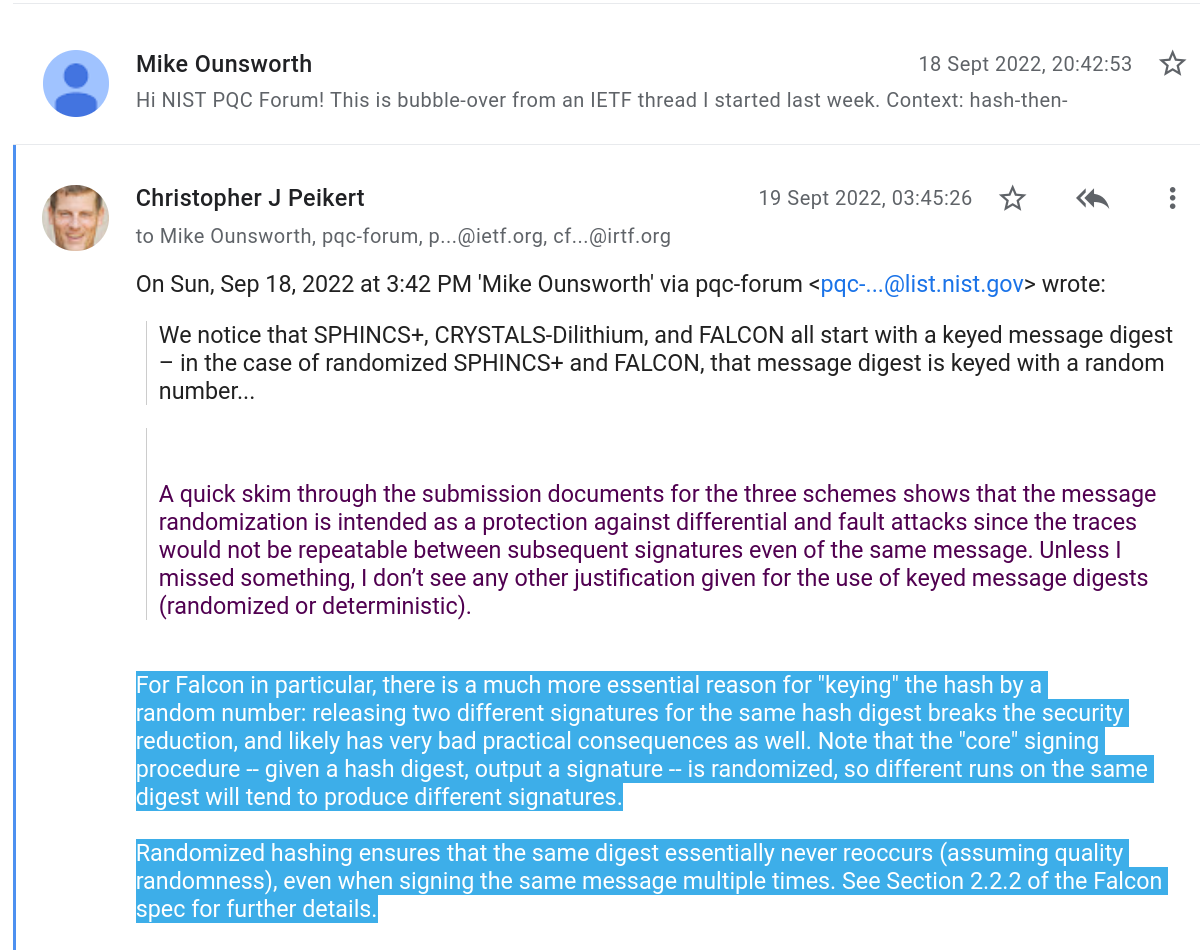
\includegraphics[keepaspectratio,frame,height=.5\textheight]{./assets/falcon-stark-warning.png}
\end{center}

Two signatures \(\vec{v}_{1}, \vec{v}_{2}\) for the same \((m,r)\) in Falcon, give \(\vec{v}_1 - \vec{v}_{2}\) s.t. \(\vec{v}_1 - \vec{v}_{2} \sim D_{\Lambda_q^\bot(\mat{A}),\sqrt{2}s,\vec{0}}\). Forgery means solving ISIS with similar norm.
\end{column}
\begin{column}[t]{0.5\columnwidth}
\begin{center}

\includegraphics[keepaspectratio,frame,height=.5\textheight]{./assets/sis-with-hints-teaser.jpg}
\end{center}

This is precisely the H-ISIS problem.
\end{column}
\end{columns}
\end{frame}
\section{Reduction}
\label{sec:org790b055}
\begin{frame}[label={sec:org1f617dd}]{Main result}
\begin{block}{Theorem}
\(\left(2^{O(n)}, \poly[n]\right)\mhyphen {}\poly[n]\mhyphen {}SIVP = \emptyset\),\\
\(\implies\) There exists \(k,\beta,s\) such that \(\left(\poly[n], \poly[n]\right)\mhyphen\HISIS_{k,n,O(n),\poly[n],\beta,s} = \emptyset\).
\end{block}
\end{frame}
\begin{frame}[label={sec:org4377ae1}]{Geometry of sieves: ``There cannot be too many points in a ball that are far apart.''}
\begin{columns}
\begin{column}{0.5\columnwidth}
\begin{lemma}[]
Let \(S \subset \ball{m}{\beta}\). \\

If \(\abs{S} > 2^{m\log(1+2\gamma)}\), there exist distinct \(\vec{c}', \vec{c}'' \in S\) with \(\norm{\vec{c}' - \vec{c}''} \leq \beta/\gamma\).
\label{lem:simple-point-bound}
\end{lemma}

\textbf{Remark:} Cost estimates for lattice schemes such as Falcon or Kyber use a heuristic variant of this theorem.
\end{column}
\begin{column}{0.5\columnwidth}
\centering
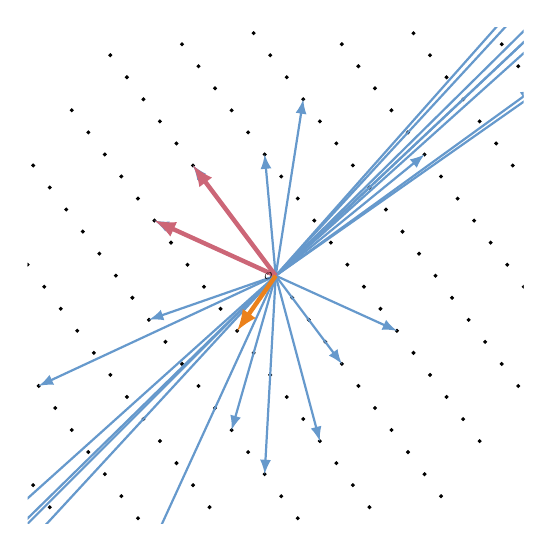
\begin{tikzpicture}[scale=0.35, every node/.style={scale=0.35}]
  \coordinate (Origin)   at (0,0);

  \clip (-9,-9) rectangle (9,9);
  \pgftransformcm{1}{0.6}{0.7}{1}{\pgfpoint{0cm}{0cm}}

  \coordinate (Bone) at (0,2);
  \coordinate (Btwo) at (2,-2);

  \foreach \x in {-10,-9,...,10}{%
    \foreach \y in {-10,-9,...,10}{%
      \node[draw,circle,inner sep=1pt,fill] at (2*\x,2*\y) {};
    }
  }

  \foreach \x in {-5,-3,2,4,5}{%
    \foreach \y in {-6,-4,1,4,5}{%
      \draw [thick,-latex,DarkBlue] (Origin)
      -- (2*\x,2*\y) {};
    }
  }

  \draw [ultra thick,-latex,LightRed] (Origin) -- (-10,10) {};
  \draw [ultra thick,-latex,LightRed] (Origin) -- (-10,8) {};
  \draw [ultra thick,-latex,LightBrown] (Origin) -- (0,-2) {};

  \node [left] at (Origin) {$\mathcal{O}$};
\end{tikzpicture}
\end{column}
\end{columns}
\end{frame}
\begin{frame}[label={sec:orgfd56e18},t]{Probabilistic upgrade}
\begin{lemma}[``No distribution over a ball can avoid close pairs.'']
For \textbf{any (malicious) distribution} \(D\) over \(\ball{m}{\beta}\) with finite support:
\[
\Pr_{\vec{c}', \vec{c}'' \gets D}\left[\norm{\vec{c}' - \vec{c}''} \leq \beta/\gamma\right] \geq \frac{1}{2^{m \log(1+2\gamma)}}.
\]
\label{lem:prob}
\end{lemma}

\pause

\begin{theorem}[{Motzkin--Straus Theorem~\cite{Motzkin_Straus_1965}}]
Let \(G\) be an undirected simple graph with adjacency matrix \(\mat{M}\).
\[
  \max_{\vec{d} \in [0,1]^n, \norm{\vec{d}}_1 = 1}\ \vec{d}^T \cdot \mat{M} \cdot \vec{d} = 1 - \frac{1}{\omega(G)}
\]
where \(\omega(G) = \max\{ \abs{X} \colon X \subseteq V \wedge (\forall (x,y \in X \wedge x \neq y),\, \{x,y\} \in E)\}\) is the clique number.
\label{thm:motzkin-straus}
\end{theorem}

\pause

Define \(G\) so that \(\vec{c}\) and \(\vec{c}'\) are connected iff \(\norm{\vec{c}'-\vec{c}''} > \beta/\gamma\). Clique = "(anti-)cluster" of far-apart points. Apply Motzkin--Straus and geometry of sieves: \(\omega(G) \leq 2^{m \log(1+2\gamma)}\).
\end{frame}
\begin{frame}[label={sec:orgcc582ed}]{A sieving algorithm}
\begin{columns}
\begin{column}[t]{0.4\columnwidth}
\centering
\procedure[linenumbering,mode=text]{$\bdv^\adv(\mat{A}, \{\vec{u}_{i}\}_{1 \leq i \leq k})$}{%
\(s \coloneqq \beta/(2\gamma\sqrt{2m})\)\\
\pcfor{up to \(2^{O(m \cdot (1 + \log 4\gamma))}\) times}\\
\pcind \(\vec{v}_{\ell}, \vec{v}_{r} \gets D_{\ZZ^m,s} \times D_{\ZZ^m,s}\)\\
\pcind \(\vec{v}'_{\ell} \gets \adv(\mat{A}, \mat{A} \cdot \vec{v}_{\ell}, \{\vec{u}_{i}\}_{1 \leq i \leq k})\)\\
\pcind \(\vec{v}'_{r} \gets \adv(\mat{A}, \mat{A} \cdot \vec{v}_{r}, \{\vec{u}_{i}\}_{1 \leq i \leq k})\)\\
\pcind \pcif {\(\norm{\vec{v}'_{\ell} - \vec{v}'_{r}} \leq \beta/(2\gamma)\)}\\
\pcind \pcind \pcreturn \((\vec{v}_{\ell}-\vec{v}_{r}) - (\vec{v}'_{\ell} - \vec{v}'_{r})\)
}
\end{column}
\begin{column}[t]{0.6\columnwidth}
\pause

\begin{itemize}
\item \(\gamma \in O(1) \implies 2^{O(m \cdot (1 + 4\gamma))} = 2^{O(m)}\)
\item \(\vec{0} \equiv \mat{A} \cdot \left(\vec{v}_{i} - \vec{v}'_{i}\right) \bmod q\) for \(i \in \{\ell,r\}\)\\
\(\implies \vec{0} \equiv \mat{A} \cdot (\vec{v}_{\ell}-\vec{v}_{r}) - (\vec{v}'_{\ell} - \vec{v}'_{r}) \bmod q\)
\item \((\vec{v}_{\ell}-\vec{v}_{r}) - (\vec{v}'_{\ell} - \vec{v}'_{r}) \approx_{s} D_{\Lambda_q^\bot(\mat{A}), \sqrt{2}s, \vec{v}'_r-\vec{v}'_\ell}\)
\end{itemize}
\end{column}
\end{columns}
\end{frame}
\begin{frame}[label={sec:org3c741bd}]{Cleaning up the output distribution}
An adaptation of \autocite{AC:DFPS22} gives us:

\begin{description}
\item[{Have}] \(Q'_{(i,j)} \coloneqq D_{\Lambda_q^\bot(\mat{A}),s,\vec{v}'_i} - D_{\Lambda_q^\bot(\mat{A}),s,\vec{v}'_j}\)
\item[{Close to}] \(Q_{(i,j)} \coloneqq D_{\Lambda_q^\bot(\mat{A}),\sqrt{2}s,\vec{v}'_i-\vec{v}'_j}\) with \(\Delta(Q'_{(i,j)}, Q_{(i,j)}) \leq 2^{-\Omega(m)}\)
\item[{Want}] \(P_{i} \coloneqq D_{\Lambda_q^\bot(\mat{A}),\sqrt{2}s,0}\)
\item[{Get}] \(P'_{i}\) with \(\Delta(P'_{i}, P_{i}) \leq 2^{-\Omega(m)}\) in \((\tau,\mu) = (2^{O(m)}, \poly[n])\)
\end{description}
\begin{alertblock}{Punchline}
We can "clean up" the distribution output by our sieve to be close to a zero-centred Gaussian like the hints but a constant factor \(\gamma\) shorter.
\end{alertblock}
\end{frame}
\begin{frame}[label={sec:orgb624547}]{Recursion}
Assume there is a chain of such \(\{\bdv_{i}\}_{1 \leq i \leq z}\).

\begin{itemize}
\item Feed the outputs of \(\bdv_{i}\) to \(\bdv_{i+1}\) as hints.
\item This allows us to make progress \(\gamma^{z} \ge 2^{\Omega(\poly[n])}\).
\item Start the chain by sampling from a discrete Gaussian with \(s_{1} \in \omega(\log m) \cdot \sqrt{m} \cdot q\) -- which is easy -- to produce the required initial hints.
\end{itemize}
\end{frame}
\begin{frame}[label={sec:org4e1827b}]{Stopping condition}
At some point, this process has to stop working, because there simply cannot be some \(\bdv_{z}\) for the required parameters, in particular \(\beta_{z}\).

\begin{itemize}
\item We establish that when
\[
  \beta_{z} \ge \Omega(m) \cdot \lambda_{m}(\Lambda_q^{\bot}(\mat{A}))
  \]
then a polynomially number of Gaussians sampled by \(\bdv_{z}\) will span the entire lattice with overwhelming probability.
\item We also establish that
\[
  \lambda_{m}(\Lambda_q^{\bot}(\mat{A})) \in O(\sqrt{\log m}) \cdot \lambda_{1}(\Lambda_q^{\bot}(\mat{A})),
  \]
suggesting that such a best-case \(\adv_{z}\) would sample solutions within a factor of \(O(m \cdot \sqrt{\log m})\) from optimal: \(\lambda_{1}(\Lambda_q^{\bot}(\mat{A}))\).
\end{itemize}
\end{frame}
\begin{frame}[label={sec:org8026d00}]{Caveats}
\begin{itemize}
\item In general, we cannot derive the existence of \(\bdv_{i+1}\) from \(\bdv_{i}\)
\item It is not a given that \(\bdv_{i}\) and \(\bdv_{i+1}\) "agree" on which \(\mat{A}\) they accept as inputs, i.e. succeed on them.
\end{itemize}
\end{frame}
\begin{frame}[label={sec:org979af07}]{Some H-ISIS must be hard if lattices are space-time hard}
For a given \(\mat{A} \gets \ZZ_{q}^{n \times m}\):

\begin{description}
\item[{Either}] The H-ISIS instances for all parameters \(\{(m,n,q,\beta_{i},s_i)\}_{1 \leq i \leq z}\) are easy,
\begin{itemize}
\item which implies SIS for \(\mat{A}\) is space-time easy,
\item which means worst-case lattice problems are space-time easy
\end{itemize}
\item[{Or}] H-ISIS is hard for at least one set of the parameters \((m,n,q,\beta_{j},s_j)\)
\begin{itemize}
\item but our reduction does not establish which \(j\), i.e. we do not formally establish that the problem does not get easier as norm bounds shrink.
\end{itemize}
\end{description}
\end{frame}
\begin{frame}[label={sec:orga69d71d},standout]{Fin}
\begin{center}

\includegraphics[keepaspectratio,height=.9\textheight]{./assets/sis-with-hints-real.jpg}
\end{center}
\end{frame}
\begin{frame}[allowframebreaks]{References}
\printbibliography[heading=none]

\IfFileExists{\jobname.tex}{\embedfile[afrelationship={/Source}]{\jobname.tex}}{}

\appendix
\end{frame}
\section{Enumeration}
\label{sec:org3b49def}
\begin{frame}[label={sec:orgd6da874}]{Enumeration I -- Pick a radius}
\begin{center}
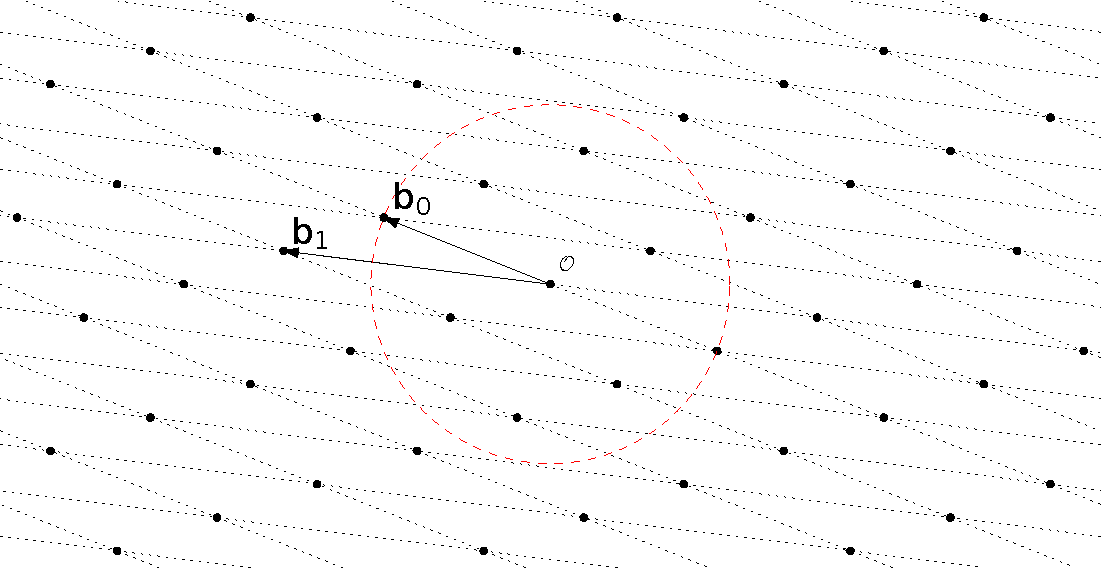
\includegraphics[width=.9\linewidth]{./assets/lattice-enumeration-0-radius.pdf}
\end{center}

{\tiny Picture credit: Joop van de Pol \par}
\end{frame}
\begin{frame}[label={sec:org1d553f5}]{Enumeration II -- Project basis}
\begin{center}
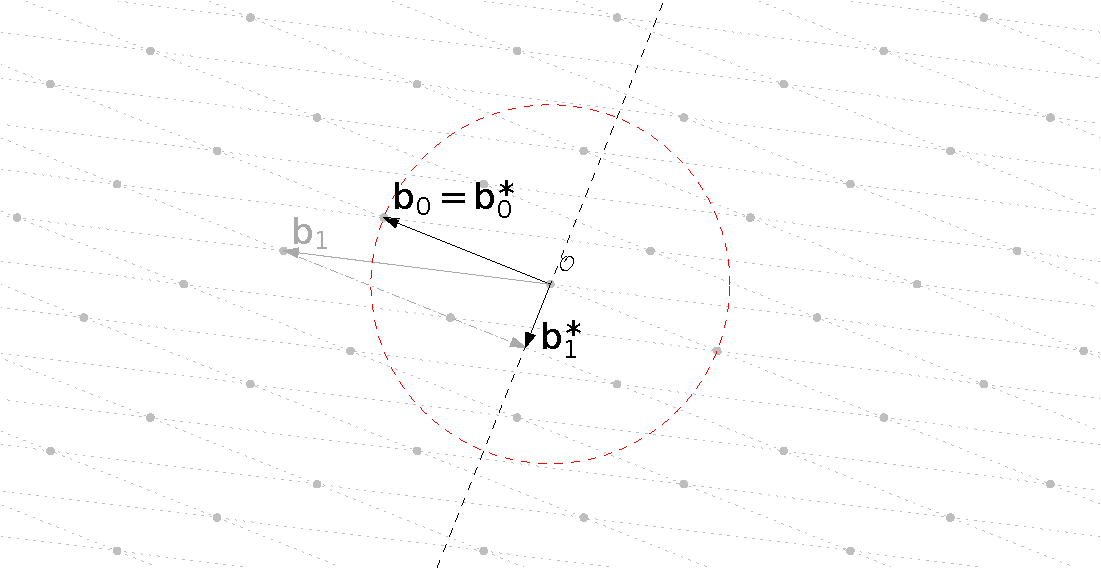
\includegraphics[width=.9\linewidth]{./assets/lattice-enumeration-1-project.pdf}
\end{center}

{\tiny Picture credit: Joop van de Pol \par}
\end{frame}
\begin{frame}[label={sec:org151c20d}]{Enumeration III -- Project lattice}
\begin{center}
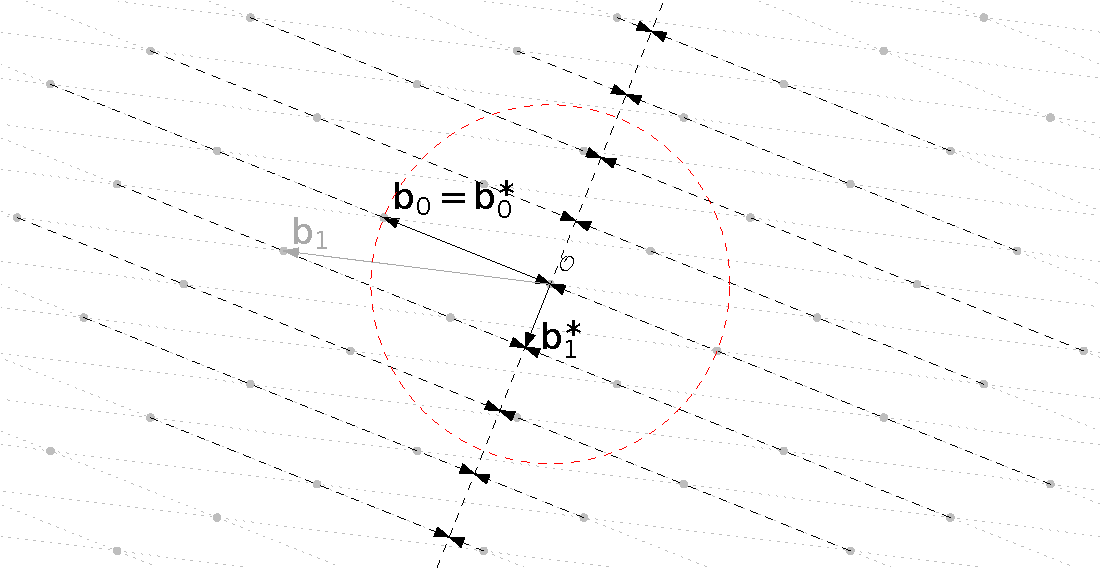
\includegraphics[width=.9\linewidth]{./assets/lattice-enumeration-2-project.pdf}
\end{center}

{\tiny Picture credit: Joop van de Pol \par}
\end{frame}
\begin{frame}[label={sec:org6b2a508}]{Enumeration IV -- Enumerate projections}
\begin{center}
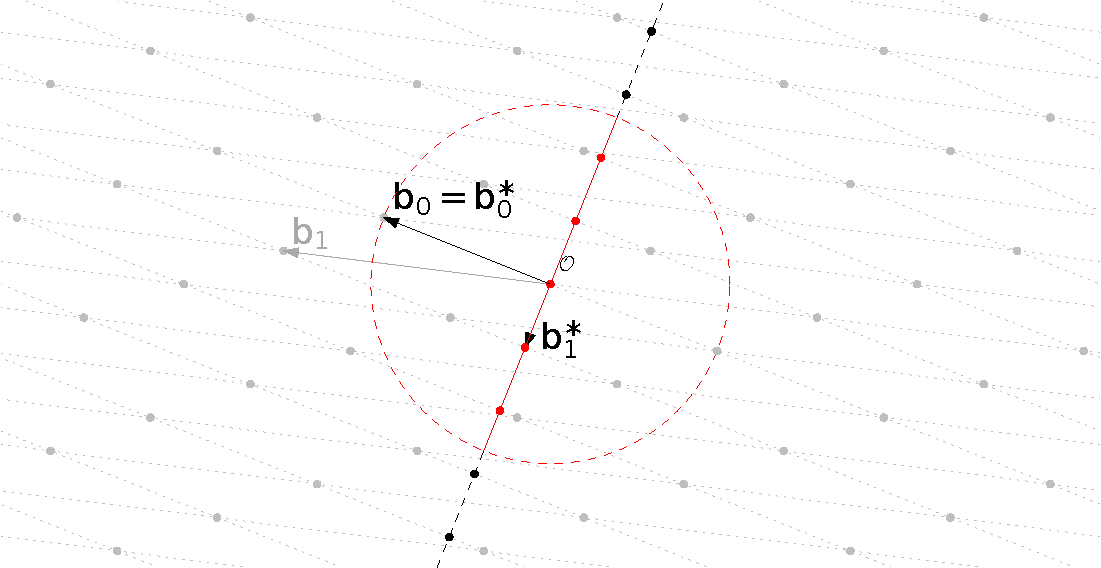
\includegraphics[width=.9\linewidth]{./assets/lattice-enumeration-3-enumerate.pdf}
\end{center}

{\tiny Picture credit: Joop van de Pol \par}
\end{frame}
\begin{frame}[label={sec:orgeda21ab}]{Enumeration V -- For each lift and enumerate}
\begin{center}
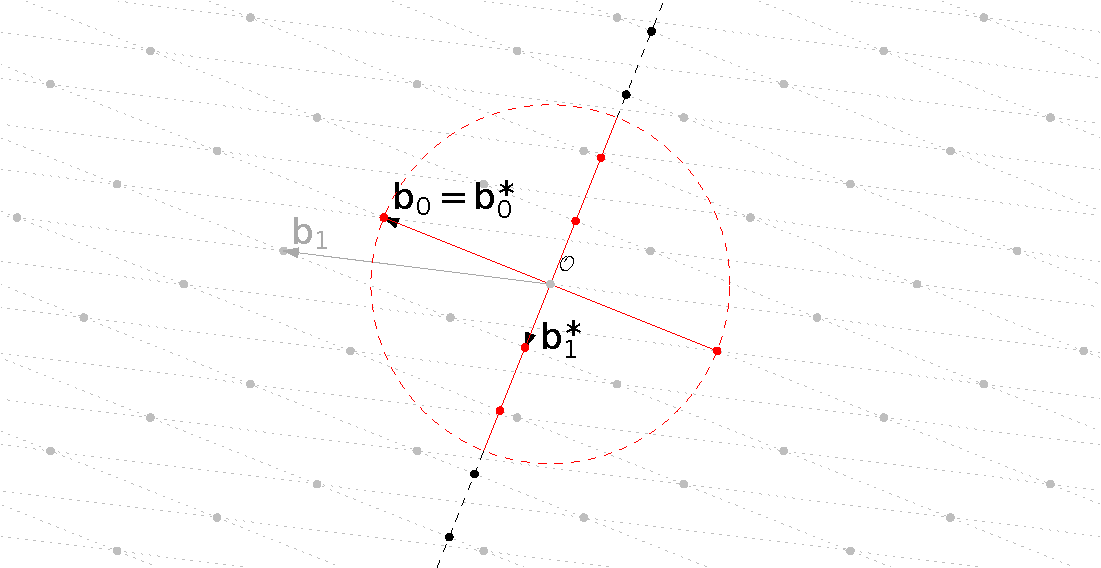
\includegraphics[width=.9\linewidth]{./assets/lattice-enumeration-4-lift.pdf}
\end{center}

{\tiny Picture credit: Joop van de Pol \par}
\end{frame}
\begin{frame}[label={sec:orgb876822}]{Enumeration V -- For each lift and enumerate}
\begin{center}
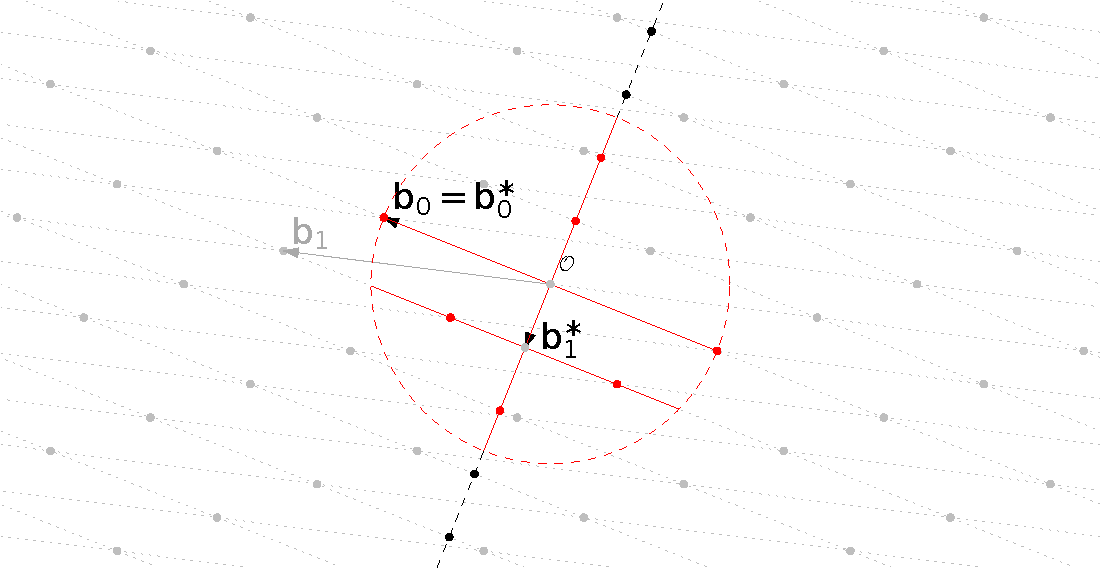
\includegraphics[width=.9\linewidth]{./assets/lattice-enumeration-5-lift.pdf}
\end{center}

{\tiny Picture credit: Joop van de Pol \par}
\end{frame}
\begin{frame}[label={sec:org55b6222}]{Enumeration VI -- Keep shortest}
\begin{center}
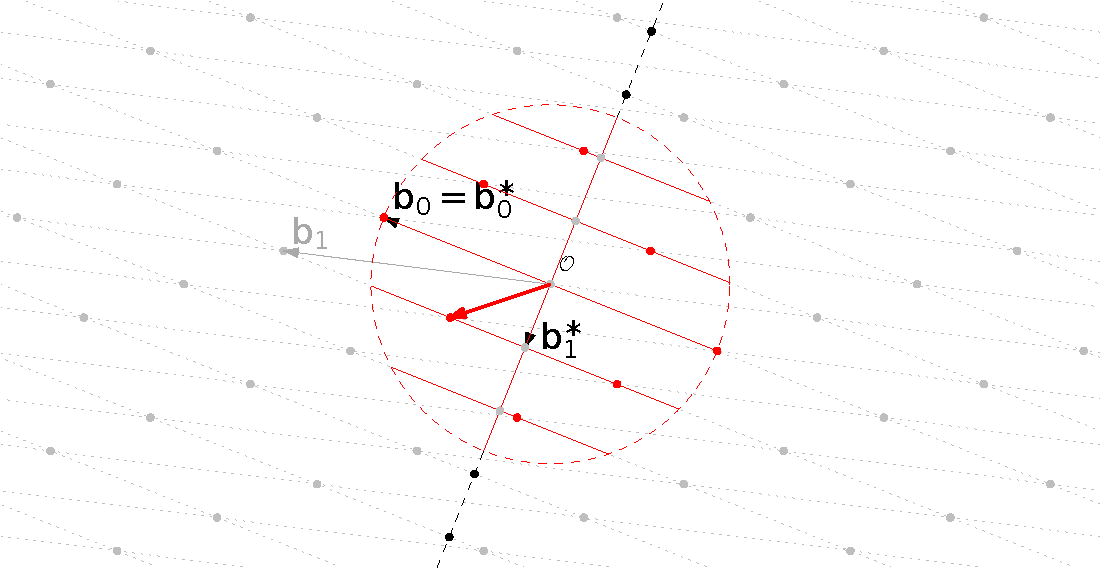
\includegraphics[width=.9\linewidth]{./assets/lattice-enumeration-6-keep.pdf}
\end{center}

{\tiny Picture credit: Joop van de Pol \par}
\end{frame}
\end{document}
